\section{Sequences of Transformations}
\label{sec:slco:sequences}

\begin{figure}[hbt]
  \centering
  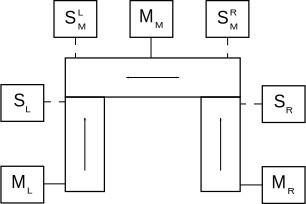
\includegraphics[scale=0.45]{slco/figs/ConveyorExampleOverview}
  \caption{Cooperating conveyor belts}
  \label{fig:ConveyorOverview}
\end{figure}

To illustrate how the transformations described in Section~\ref{sec:slco:model-transformations} can be applied, we introduce a system of three cooperating conveyor belts, schematically depicted in Figure~\ref{fig:ConveyorOverview}.
We show how different implementations for controlling this system can be generated by composing a number of transformations into different sequences of transformations.
The two vertical rectangles in Figure~\ref{fig:ConveyorOverview} denote conveyor belts that transport items towards another conveyor belt, which is represented by a horizontal rectangle.
The arrows in the rectangles denote the directions in which these conveyor belts can transport items.
The three belts should cooperate such that items supplied by the vertical belts are dropped onto the horizontal belt, one by one.
The horizontal belt should transport each of these items from the right-most belt to the left and those from the left-most belt to the right.
The small rectangles labeled~\Motor{L}, \Motor{M}, and~\Motor{R} depict the motors that drive the conveyor belts, and the small rectangles labeled~\Sensor{L}{}, \Sensor{M}{L}, \Sensor{M}{R}, and~\Sensor{R}{} depict the sensors that detect the passing items.

\begin{figure}[hbt]
  \centering
  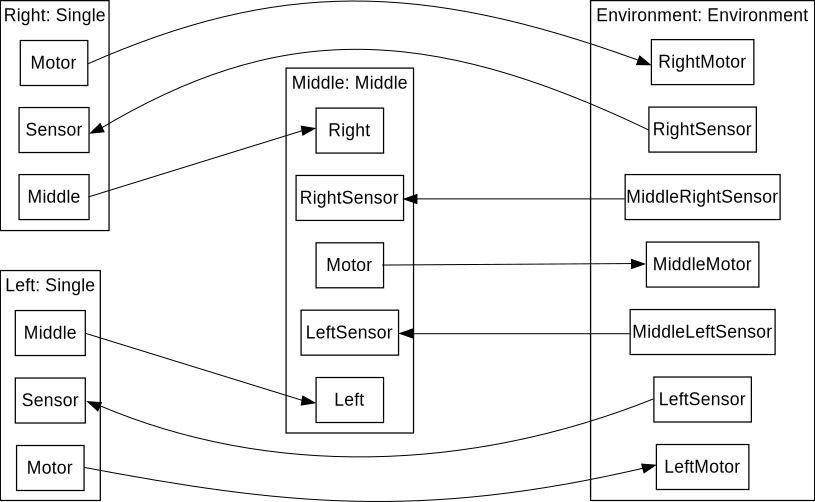
\includegraphics[scale=0.45]{slco/figs/ConveyorExampleCommunication}
  \caption{Communication between the controllers and the environment}
  \label{fig:slco:ConveyorComm}
\end{figure}

An \SLCO model that describes this system consists of four components: two objects~(\SLCOObject{Left} and~\SLCOObject{Right}) that model the controllers for the vertical belts, one object~(\SLCOObject{Middle}) that models the controller for the horizontal belt, and one object~(\SLCOObject{Environment}) that models the environment.
The communication diagram in Figure~\ref{fig:slco:ConveyorComm} shows how these objects are connected.
Among other things, it also shows that the objects~\SLCOObject{Left} and~\SLCOObject{Right} are both instances of class~\SLCOClass{Single}.
To increase the readability of the figure, the names of the channels have been omitted.

\begin{figure}[hbt]
  \centering
  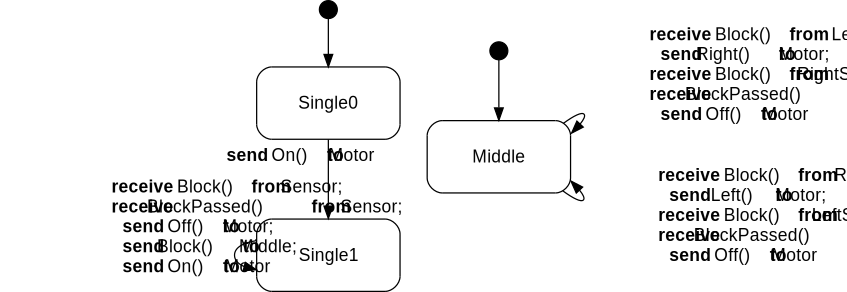
\includegraphics[scale=0.45]{slco/figs/ConveyorExampleSMS}
  \caption{Behavior of controllers}
  \label{fig:slco:ConveyorSMS}
\end{figure}

Figure~\ref{fig:slco:ConveyorSMS} shows the two state machines that specify the behavior of the controllers of this system.
The state machine on the left specifies the behavior of objects~\SLCOObject{Left} and~\SLCOObject{Right}, and the state machine on the right specifies the behavior of object~\SLCOObject{Middle}.
The state machines related to the environment are not shown.

In Figure~\ref{fig:TransformationSequences}, three sequences of model transformations leading to three distinct implementations with the same observable behavior are shown.
In this figure, \SLCO models are represented by the rectangles labeled~\SLCOModel{1} to~\SLCOModel{16}, \NQC implementations by rectangles labeled~\NQCCode{1} to~\NQCCode{3}, single transformations by labeled, solid arrows, and subsequences of transformation by labeled, dashed arrows.
The starting point of all three sequences, model~\SLCOModel{1}, describes the intended cooperation in terms of objects~\SLCOObject{Left}, \SLCOObject{Middle}, \SLCOObject{Right}, and their hardware environment.

The topmost sequence of transformations in Figure~\ref{fig:TransformationSequences} transforms the \SLCO model~\SLCOModel{1} to the \NQC implementation~\NQCCode{2}, which is meant to be deployed on two controllers.
First, objects~\SLCOObject{Left} and~\SLCOObject{Right} are merged, and the channels that connect these objects to~\SLCOObject{Middle} are also merged.
To be able to distinguish the origin of signals after merging the channels, transformation~\Transformation{ic} is applied before merging the channels.
Then, synchronous communication is replaced by asynchronous communication, after which lossless communication over a lossy channel is achieved by adding objects that implement the CABP.
Because this last transformation adds a number of objects to the model and the resulting model~\SLCOModel{8} should only contain as many objects as there are controllers, these objects must be merged with others to reduce the total number of objects again.
As mentioned above, objects can only be merged if all pairs of state machines involved in communication communicate over distinct channels.
This explains why transformation~\Transformation{ex} is applied before transformation~\Transformation{merge} is used to reduce the number of objects.
In the final transformation step, all string constants are replaced by integer constants, leading to model~\SLCOModel{8}.
Because all semantic gaps and platform gaps have been bridged, transforming this model into implementation~\NQCCode{2} using transformation~\Transformation{NQC} is straightforward.

\begin{figure}[hbt]
 \centering
 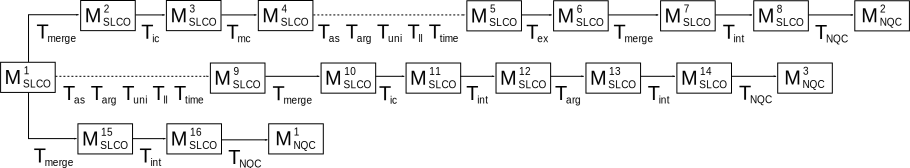
\includegraphics[scale=0.52]{slco/figs/transformations/sequences}
 \caption{Sequences of transformations}
 \label{fig:TransformationSequences}
\end{figure}

The sequence of transformations in the middle of Figure~\ref{fig:TransformationSequences} leads to an implementation with three controllers.
Because the three controllers communicate by broadcasting signals, the origin of signals has to be made explicit using transformation~\Transformation{ic}.
After applying this transformations, the names of the signals have to be changed again, and all string constant have to be replaced by integer constants, to be able to apply transformation~\Transformation{NQC}.
Transformation~\Transformation{NQC} encodes the arguments of signals into a single integer, as discussed in Section~\ref{sec:slco:transformation-to-nqc}.
To keep the number of distinct integer constants as low as possible and achieve an optimal encoding of the signal arguments, transformation~\Transformation{int} is applied both before and after transformation~\Transformation{arg}.

The sequence of transformations in the bottom of Figure~\ref{fig:TransformationSequences} generates an implementation for a system with only one controller. Therefore, all objects are merged in the first transformation step. 